\documentclass[11pt,a4paper]{article}

\usepackage[margin=2.5cm]{geometry}
\usepackage[T1]{fontenc}
\usepackage{lmodern}
\usepackage{microtype}
\usepackage{graphicx}
\usepackage{booktabs}
\usepackage{tabularx}
\usepackage{multirow}
\usepackage{amsmath}
\usepackage{xcolor}
\usepackage{listings}
\usepackage{tikz}
\usetikzlibrary{arrows.meta,positioning,shapes.geometric,fit,calc}
\usepackage{caption}
\usepackage{enumitem}
\usepackage{float}
\usepackage[hidelinks]{hyperref}

\definecolor{stock}{HTML}{C0392B}
\definecolor{patched}{HTML}{1F5FA8}
\definecolor{codebg}{HTML}{F7F7F7}
\definecolor{addline}{HTML}{1E7B34}
\definecolor{delline}{HTML}{B31D28}

\captionsetup{font=small,labelfont=bf}
\setlist{itemsep=2pt,topsep=4pt}
\setcounter{tocdepth}{2}
\emergencystretch=1.5em

\lstdefinestyle{c}{
  language=C, basicstyle=\ttfamily\footnotesize, backgroundcolor=\color{codebg},
  frame=single, rulecolor=\color{black!20}, keywordstyle=\color{patched}\bfseries,
  commentstyle=\color{black!55}\itshape, columns=fullflexible, keepspaces=true,
  showstringspaces=false, breaklines=true, xleftmargin=4pt, xrightmargin=4pt,
  aboveskip=6pt, belowskip=6pt, morekeywords={uint32_t,uint64_t,BOOLEAN,_In_,const}}
\lstdefinestyle{diff}{
  basicstyle=\ttfamily\footnotesize, backgroundcolor=\color{codebg}, frame=single,
  rulecolor=\color{black!20}, columns=fullflexible, keepspaces=true, breaklines=true,
  xleftmargin=4pt, xrightmargin=4pt, aboveskip=6pt, belowskip=6pt,
  moredelim=[il][\color{addline}]{+}, moredelim=[il][\color{delline}]{-}}
\lstset{style=c}
\makeatletter\newcommand{\inputrows}[1]{\@@input #1 }\makeatother

\newcommand{\maxfs}{\ensuremath{\mathit{maxFS}}}
\newcommand{\cwnd}{\ensuremath{\mathit{cwnd}}}
\newcommand{\ssthresh}{\ensuremath{\mathit{ssthresh}}}
\newcommand{\smss}{\ensuremath{\mathit{SMSS}}}
\newcommand{\fs}{\ensuremath{\mathit{FlightSize}}}
\newcommand{\stock}{\textcolor{stock}{\textbf{stock}}}
\newcommand{\patched}{\textcolor{patched}{\textbf{patched}}}

\begin{document}

%======================================================================
\begin{titlepage}
\centering
\vspace*{2.5cm}
{\Large Wireless Networks --- Course Project\par}
\vspace{1.5cm}
{\huge\bfseries Rate-Limited Sender Increase\\[4pt] in MsQuic CUBIC\par}
\vspace{0.8cm}
{\large Implementing and evaluating\\ \texttt{draft-ietf-ccwg-ratelimited-increase-11}\par}
\vspace{2cm}
{\large Abhiram Suresh\par}
\vspace{0.5cm}
{\large November 2026\par}
\vfill
\begin{minipage}{0.85\textwidth}
\small
\textbf{Code.} MsQuic branch \texttt{rate-limited-increase}
(commits \texttt{dd0428a62}, \texttt{19538311e}, \texttt{7c6397cf3} and the
upstream bug fix \texttt{1ca13e9d7}),
on top of upstream \texttt{464c873c0}. Patch files are in
\texttt{patches/}; experiment scripts in \texttt{experiments/};
everything needed to rebuild this document and its figures is in \texttt{report/}.
\end{minipage}
\vspace{1cm}
\end{titlepage}

%======================================================================
\begin{abstract}
\noindent
A \emph{rate-limited} sender is one that is not using its whole congestion
window: a video player between segments, an RPC client, a game, a heartbeat.
CUBIC grows the congestion window (\cwnd) with time and on every
acknowledgement, so a rate-limited sender can keep growing \cwnd\ although the
network never carried that much of its data. When the application later has a
lot to send, it releases the whole inflated window at once and overflows the
bottleneck queue. The IETF draft \emph{Increase of the Congestion Window when the
Sender Is Rate-Limited} bounds \cwnd\ by the largest flight used since the last
window reduction, \maxfs. MsQuic's CUBIC had such a bound with two gaps:
\maxfs\ was never reset, and the bound was $2\cdot\maxfs$ in congestion
avoidance too. We close both gaps (34 lines of code, four new unit tests) and
show with a deterministic ablation that each of our five changes matters.
Evaluating the patch on an emulated bottleneck (420 runs, 11 settings) we also
found an \emph{upstream bug}: an unsigned underflow in CUBIC's Reno-friendly
accumulator that makes \cwnd\ grow by one packet per ACK in congestion
avoidance; we fix it as well. With the bug fixed in both builds, after 28\,s
of rate-limited sending our change cuts \cwnd\ at resumption from 670 to
166\,KB and the data lost after resuming from 1094 to 32\,KB, at no cost in
transfer time; in shorter periods it still cuts losses by 34--63\,\%. The
patch needs the bug fix: without it, a competing TCP flow can stall. On a
50\,Mbit/s path with a shallow queue the conservative window costs 23\,\% in
completion time of the following 8\,MB transfer.
\end{abstract}

{\small\tableofcontents}
\newpage

%======================================================================
\section{Introduction: why this matters}
\label{sec:intro}

Most real Internet traffic is not a long bulk transfer. It comes in bursts
separated by quiet periods, and between the bursts the sender has less to
send than its congestion window would allow. Examples:
\begin{itemize}
  \item \textbf{Adaptive video.} A player downloads a few seconds of video,
        then waits for the buffer to drain, then downloads again.
  \item \textbf{Request/response protocols} (HTTP/3, RPC). The sender is
        limited by how fast requests arrive, not by the network.
  \item \textbf{Real-time and interactive traffic} (games, telemetry,
        heartbeats). The sender emits a few small packets per round trip.
\end{itemize}

The congestion window exists to answer one question: \emph{how much data can
this path safely carry right now?} The only evidence the sender has is the
data it actually sent and got acknowledged. If the sender keeps only 29\,KB
in flight but lets \cwnd\ grow to 400\,KB, the extra 371\,KB is a guess
nobody checked. The problem shows up when the application suddenly has a lot
to send (the next video chunk, a large response): the sender is allowed to
release the whole window in one round trip. That burst lands in the
bottleneck queue, the queue overflows, packets of \emph{other} flows are
dropped and their latency jumps.

Figure~\ref{fig:hook} shows the problem on a real network stack
(Section~\ref{sec:net}). After a loss, the application sends only about
25\,KB per round trip for 28\,s. Stock MsQuic's CUBIC keeps growing \cwnd\
until it hits a limit computed from a flight it last used half a minute
earlier: 670\,KB, 27 times what is in flight. When the application then has
8\,MB to send, the whole window leaves at once and about 1.1\,MB is lost.
The patched sender keeps \cwnd\ at what it has used and loses 24\,KB in
this run (median over 10 runs: 32\,KB against 1094\,KB).

\begin{figure}[ht]
  \centering
  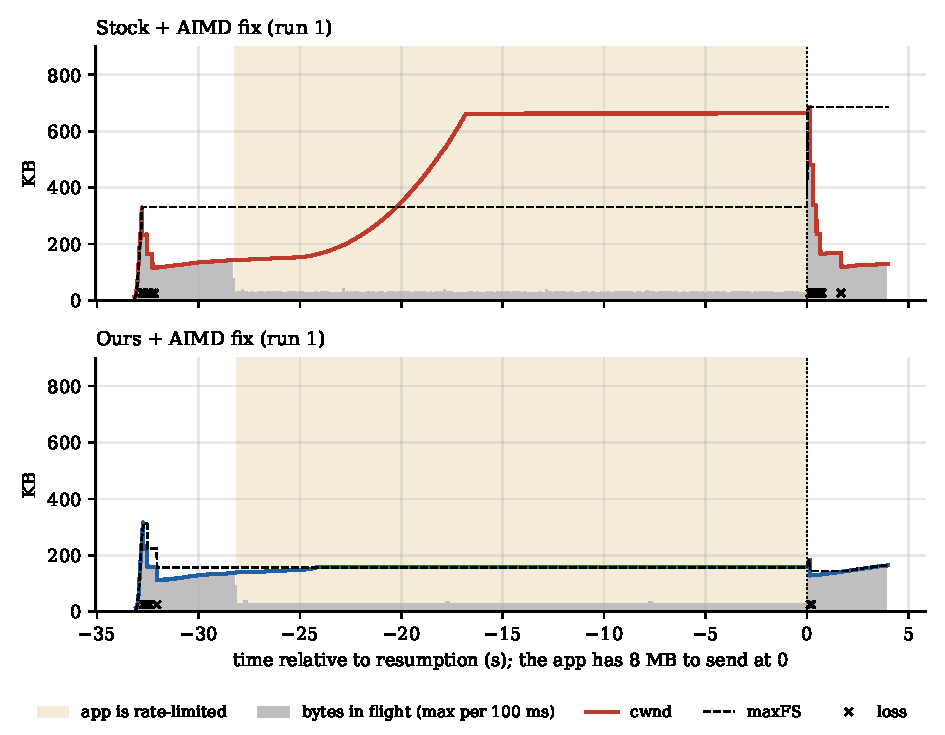
\includegraphics[width=\textwidth]{figures/clean_timeline.pdf}
  \caption{One run of the 28\,s rate-limited setting. The AIMD bug of
    Section~\ref{sec:bug} is fixed in both builds, which changes nothing in this
    setting, so the difference is the draft's rule alone. x: loss detected.}
  \label{fig:hook}
\end{figure}

\paragraph{Contributions.}
\begin{enumerate}
  \item An analysis of where MsQuic's CUBIC deviates from the draft (two gaps,
        Section~\ref{sec:gaps}).
  \item A patch that closes both gaps, made of five small changes C1--C5
        (Section~\ref{sec:impl}), plus four new and two updated unit tests.
  \item A deterministic scenario harness and an ablation study that shows,
        for \emph{each} change separately, the situation in which it matters
        and what goes wrong without it (Section~\ref{sec:examples}).
  \item The discovery and fix of an upstream bug in MsQuic's CUBIC, the
        underflow of the Reno-friendly accumulator (Section~\ref{sec:bug}).
  \item A testbed evaluation with 420 runs: a sweep over the length of the
        rate-limited period, RTT, bottleneck rate and a competing TCP flow, and a
        four-build experiment that separates the effect of our change from that
        of the bug (Section~\ref{sec:net}).
\end{enumerate}

%======================================================================
\section{Background}
\label{sec:bg}

\subsection{Congestion window, flight size and slow start}

The sender may have at most \cwnd\ bytes unacknowledged. \fs\ is the number
of bytes actually in flight. A sender is \emph{cwnd-limited} when
$\fs \approx \cwnd$ and \emph{rate-limited} (also called application-limited)
when $\fs < \cwnd$ because the application has nothing more to send.
In \emph{slow start} ($\cwnd < \ssthresh$) the window doubles every round
trip; in \emph{congestion avoidance} ($\cwnd \ge \ssthresh$) it grows slowly.
On a loss or ECN mark the window is reduced (by CUBIC's $\beta = 0.7$) and
\ssthresh\ is set to the new window.

\subsection{Why CUBIC is especially exposed}

CUBIC (RFC~9438) computes the window as a function of \emph{time since the
last congestion event}, $W(t) = C\,(t-K)^3 + W_{\max}$, not as a function of
the number of ACKs. As long as ACKs keep arriving, the window follows this
curve. A rate-limited sender still receives ACKs (for its few packets), so
the window climbs the cubic curve exactly as if the path had been fully used.
The longer the rate-limited period, the larger the unvalidated window. In our
testbed the window grew from 150\,KB to 670\,KB during 28\,s in which only
about 25\,KB was ever in flight (Figure~\ref{fig:hook}).

\subsection{The draft's rules}

\texttt{draft-ietf-ccwg-ratelimited-increase-11} updates RFC~5681, RFC~9002
and others with a simple rule. It introduces
\[
  \maxfs = \text{the largest \fs\ since the last time \cwnd\ was reduced,}
\]
and requires that, while rate-limited, the window does not grow past what
\maxfs\ justifies:

\begin{table}[ht]
\centering
\caption{The rules of the draft that this project implements.}
\label{tab:rules}
\begin{tabularx}{\textwidth}{@{}l X@{}}
\toprule
\textbf{Rule} & \textbf{Requirement} \\
\midrule
R1 Reset & When \cwnd\ is reduced for any reason, \maxfs\ is reset to 0 and
           re-measured from the following \fs. \\
R2 Slow start & $\cwnd \le 2\cdot\maxfs$ (allows one doubling over what was used). \\
R3 Congestion avoidance & $\cwnd \le \maxfs + 1\cdot\smss$ (allows the normal
           one-packet-per-RTT probe over what was used). \\
\bottomrule
\end{tabularx}
\end{table}

These rules are the successor to Congestion Window Validation (RFC~7661),
which instead \emph{decays} \cwnd\ after idle/rate-limited periods. The draft
takes the simpler approach of never letting the window run ahead of the
evidence in the first place.

%======================================================================
\section{What stock MsQuic does, and the two gaps}
\label{sec:gaps}

MsQuic's CUBIC (\texttt{src/core/cubic.c}) already tracks \maxfs\ in a
field called \texttt{BytesInFlightMax}. It is updated on every send
(\texttt{OnDataSent}) and is used at the end of
\texttt{OnDataAcknowledged} to cap the window:

\begin{lstlisting}[title={\footnotesize Stock \texttt{cubic.c}, end of \texttt{OnDataAcknowledged}}]
    // Using 2 * BytesInFlightMax for the limit allows for exponential growth
    // in the window when not otherwise limited.
    if (Cubic->CongestionWindow > 2 * Cubic->BytesInFlightMax) {
        Cubic->CongestionWindow = 2 * Cubic->BytesInFlightMax;
    }
\end{lstlisting}

The field is set to $\cwnd/2$ at initialisation and on reset, and
otherwise only ever grows. (The draft initialises \maxfs\ to the initial
window instead; we kept MsQuic's value, see Section~\ref{sec:disc}.) Compared with Table~\ref{tab:rules}:

\begin{description}
  \item[Gap 1: \maxfs\ is never reset (violates R1).] After a loss the window
        is cut to 70\,\%, but \maxfs\ keeps the pre-loss peak. The cap
        $2\cdot\maxfs$ is then computed from a flight size that the network
        just showed it \emph{cannot} carry.
  \item[Gap 2: the congestion-avoidance cap is $2\cdot\maxfs$ (violates R3).]
        In congestion avoidance the window may be twice the largest flight,
        instead of one packet more than it.
\end{description}

\subsection{A worked example of both gaps}
\label{sec:worked}

Take the situation of Scenario~A (Section~\ref{sec:scenA}). Units are
packets of 1232\,B.
\begin{enumerate}
  \item The sender is cwnd-limited and reaches $\cwnd = 40$, with 40 packets
        in flight. So $\maxfs = 40$.
  \item 12 of the 40 are lost. CUBIC cuts the window to
        $\cwnd = \ssthresh = 0.7\cdot 40 = 28$.
  \item The application now sends only 4 packets per RTT for 10 seconds
        (200 RTTs of 50\,ms).
\end{enumerate}

\begin{table}[ht]
\centering
\caption{Window limits in the worked example after the loss. With stock
  MsQuic, CUBIC's time-driven growth fills all the headroom it is allowed.}
\label{tab:worked}
\begin{tabular}{@{}lccc@{}}
\toprule
 & \maxfs\ after loss & cap in CA & \cwnd\ after 10\,s \\
 & & & at 4 pkt/RTT \\
\midrule
Stock (Gap 1 + Gap 2) & 40 (stale) & $2\cdot 40 = 80$ & \textbf{76.5} \\
Draft rules & $0\to 28$ (reset, re-measured) & $28 + 1 = 29$ & \textbf{29} \\
\bottomrule
\end{tabular}
\end{table}

With stock MsQuic the sender ends up with a 76-packet window, \emph{bigger
than the 40 packets that just caused a loss}, although it never had more
than 4 packets in flight after the loss. When the application resumes, all
76 packets go out in one round trip.

%======================================================================
\section{Implementation}
\label{sec:impl}

The patch adds 34 lines of code and 30 lines of comments to \texttt{cubic.c}
and \texttt{cubic.h} (one new field), not counting the experiment-only trace
logger of Section~\ref{sec:instr}. It consists of five changes.
Figure~\ref{fig:hooks} shows where each one sits in the CUBIC callbacks.

\begin{figure}[ht]
\centering
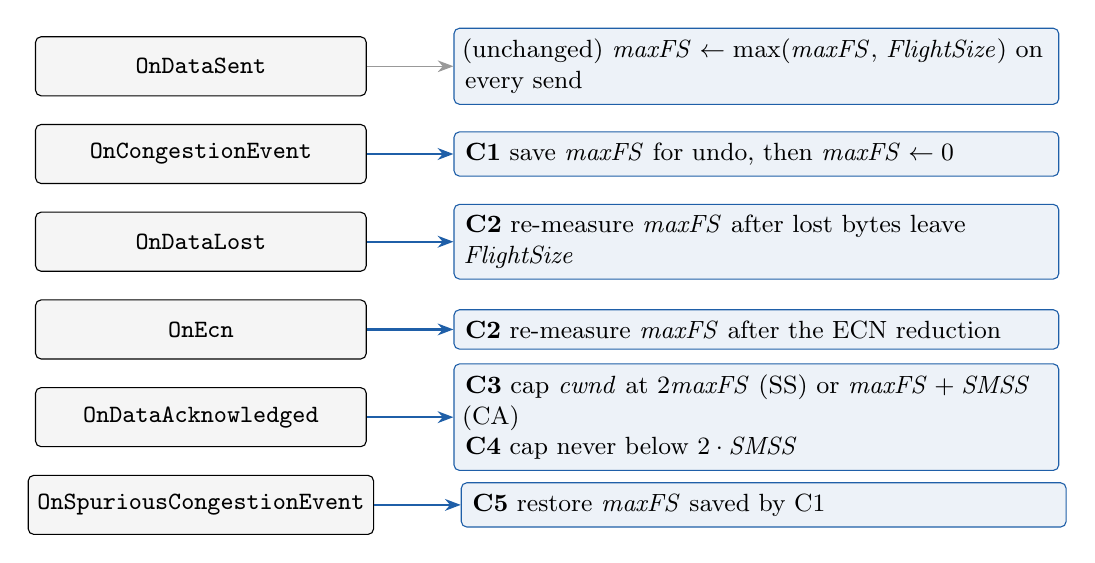
\begin{tikzpicture}[
    cb/.style={draw, rounded corners=2pt, minimum width=4.2cm, minimum height=0.75cm,
               font=\ttfamily\small, fill=black!4},
    ch/.style={draw=patched, fill=patched!8, rounded corners=2pt, text width=7.4cm,
               font=\small, inner sep=4pt, align=left},
    lnk/.style={-{Stealth[length=2mm]}, patched, thick},
    node distance=0.35cm]
  \node[cb] (sent) {OnDataSent};
  \node[cb, below=of sent] (cong) {OnCongestionEvent};
  \node[cb, below=of cong] (lost) {OnDataLost};
  \node[cb, below=of lost] (ecn) {OnEcn};
  \node[cb, below=of ecn] (ack) {OnDataAcknowledged};
  \node[cb, below=of ack] (spur) {OnSpuriousCongestionEvent};

  \node[ch, right=1.1cm of sent] (n0) {(unchanged) $\maxfs \leftarrow \max(\maxfs,\,\fs)$ on every send};
  \node[ch, right=1.1cm of cong] (c1) {\textbf{C1} save \maxfs\ for undo, then $\maxfs \leftarrow 0$};
  \node[ch, right=1.1cm of lost] (c2a) {\textbf{C2} re-measure \maxfs\ after lost bytes leave \fs};
  \node[ch, right=1.1cm of ecn] (c2b) {\textbf{C2} re-measure \maxfs\ after the ECN reduction};
  \node[ch, right=1.1cm of ack] (c3) {\textbf{C3} cap $\cwnd$ at $2\maxfs$ (SS) or $\maxfs+\smss$ (CA)\\
                                      \textbf{C4} cap never below $2\cdot\smss$};
  \node[ch, right=1.1cm of spur] (c5) {\textbf{C5} restore \maxfs\ saved by C1};
  \draw[black!40, -{Stealth[length=2mm]}] (sent) -- (n0);
  \foreach \a/\b in {cong/c1, lost/c2a, ecn/c2b, ack/c3, spur/c5} \draw[lnk] (\a) -- (\b);
\end{tikzpicture}
\caption{The CUBIC callbacks and the change made in each
  (\texttt{OnDataLost} and \texttt{OnEcn} both call \texttt{OnCongestionEvent}). Blue boxes are new
  behaviour; the grey box is existing behaviour the patch relies on.}
\label{fig:hooks}
\end{figure}

\subsection*{C1 --- reset \maxfs\ on every congestion event (closes Gap 1)}

\texttt{CubicCongestionControlOnCongestionEvent} is the single place where
CUBIC reduces the window for loss, ECN and persistent congestion, so one
line there implements R1 for all of them. The old value is saved first so
that a spurious loss can be undone (C5).

\begin{lstlisting}[style=diff]
+        Cubic->PrevBytesInFlightMax = Cubic->BytesInFlightMax;
     ...
+    // "upon a reduction of cwnd (for any reason), maxFS MUST be reset to zero"
+    Cubic->BytesInFlightMax = 0;
\end{lstlisting}

\subsection*{C2 --- re-measure \maxfs\ right after the reduction}

After a reset to 0, the draft says \maxfs\ is measured again from the next
\fs. If we waited for the next \texttt{OnDataSent}, any ACK arriving before
that would see $\maxfs = 0$. So both callers of the congestion event measure
it immediately, at the point where \fs\ is already correct:
in \texttt{OnDataLost} \emph{after} the lost bytes have been subtracted
(otherwise lost packets would count as ``carried''), and in \texttt{OnEcn}
after the reduction.

\begin{lstlisting}
static void
CubicCongestionControlUpdateMaxFlightSize(_In_ QUIC_CONGESTION_CONTROL_CUBIC* Cubic)
{
    if (Cubic->BytesInFlightMax < Cubic->BytesInFlight) {
        Cubic->BytesInFlightMax = Cubic->BytesInFlight;
    }
}
\end{lstlisting}

\subsection*{C3 --- a phase-dependent cap (closes Gap 2), and C4 --- a floor}

\begin{lstlisting}[style=diff]
-    if (Cubic->CongestionWindow > 2 * Cubic->BytesInFlightMax) {
-        Cubic->CongestionWindow = 2 * Cubic->BytesInFlightMax;
-    }
+    const uint32_t Smss = QuicPathGetDatagramPayloadSize(&Connection->Paths[0]);
+    const BOOLEAN InSlowStart = Cubic->CongestionWindow < Cubic->SlowStartThreshold;
+    uint32_t CwndLimit;
+    if (InSlowStart) {
+        CwndLimit = 2 * Cubic->BytesInFlightMax;          // R2
+    } else {
+        CwndLimit = Cubic->BytesInFlightMax + Smss;       // R3
+    }
+    const uint32_t MinWindow = Smss * QUIC_PERSISTENT_CONGESTION_WINDOW_PACKETS;
+    if (CwndLimit < MinWindow) {                         // C4
+        CwndLimit = MinWindow;
+    }
+    if (Cubic->CongestionWindow > CwndLimit) {
+        Cubic->CongestionWindow = CwndLimit;
+    }
\end{lstlisting}

C4 is not in the draft's text but is required by QUIC: RFC~9002 says the
window must never go below the minimum window of 2 packets
(\texttt{QUIC\_PERSISTENT\_CONGESTION\_WINDOW\_PACKETS}). Without it, a sender
whose flight is a single small packet would get a window smaller than one
full packet (Scenario~D).

\subsection*{C5 --- restore \maxfs\ when a loss turns out to be spurious}

MsQuic undoes a congestion event when the ``lost'' packets are acknowledged
after all. It already restored \cwnd, \ssthresh\ and the CUBIC state from
\texttt{Prev*} copies. Because C1 now changes \maxfs\ on the congestion event,
it has to be restored too, otherwise the first ACK after the undo would cap
the restored window with the post-loss \maxfs\ (Scenario~C).

\begin{lstlisting}[style=diff]
+    uint32_t PrevBytesInFlightMax;                   // cubic.h
+    Cubic->BytesInFlightMax = Cubic->PrevBytesInFlightMax;   // OnSpuriousCongestionEvent
\end{lstlisting}

\subsection{A design decision: \ssthresh\ is left alone}
\label{sec:design}

When C3 lowers the window below \ssthresh, the sender is technically back
in slow start, and on the next ACK the slow-start cap $2\cdot\maxfs$ applies,
so \cwnd\ can rise again until it reaches \ssthresh. The window therefore
oscillates, but always within $\min(\ssthresh, 2\cdot\maxfs)$.

An earlier version of the patch also lowered \ssthresh\ to the capped
window to stop the oscillation. The ablation (Scenario~B and~D) showed this
is harmful: \ssthresh\ is the sender's memory of the last \emph{real}
congestion, and lowering it without any congestion signal makes the sender
leave slow start early when the application later becomes cwnd-limited.
In Scenario~D, the sender sent 23 packets in the 15th RTT with \ssthresh\
untouched and only 9 with it lowered (Figure~\ref{fig:scenD}). The draft
also does not ask for it. We therefore reverted it (commit
\texttt{7c6397cf3}). All network results are for the final version. In the
testbed the cap pushed \cwnd\ below \ssthresh, where the rejected variant would
have acted, only in 2 of 10 runs per build of the competing-TCP setting and in
no run of any other setting.

\subsection{Instrumentation}
\label{sec:instr}

For the experiments, a CSV logger (\texttt{CUBIC\_CWND\_LOG}) records
\cwnd, \maxfs, \fs\ and \ssthresh\ at every send, ACK and loss. It is
compiled only with \texttt{-DQUIC\_CUBIC\_CWND\_LOG} and has no effect on
normal builds. The sample client (\texttt{src/tools/sample/sample.c}) gained
options to produce a controlled rate-limited workload
(\texttt{-prime}, \texttt{-burst}, \texttt{-pause}, \texttt{-cycles},
\texttt{-final}) and prints the connection statistics at the end.

%======================================================================
\section{Per-change examples: the scenario harness and ablation}
\label{sec:examples}

Network experiments show the overall effect but cannot tell which change is
responsible, and they are noisy. To show precisely \emph{where} each change
matters, we drive CUBIC directly through its callbacks inside MsQuic's own
unit-test harness. Every scenario is a deterministic script of sends, ACKs
and losses (one round = one 50\,ms RTT, $\smss = 1232$\,B, HyStart off),
and is run against seven builds of \texttt{cubic.c}:

\begin{table}[ht]
\centering
\caption{Builds used in the ablation. Each ``no\_'' build is the final patch
  with exactly one change switched off by a compile-time macro.}
\label{tab:variants}
\begin{tabular}{@{}ll@{}}
\toprule
Build & Meaning \\
\midrule
\textcolor{stock}{stock} & upstream \texttt{cubic.c} \\
\textcolor{patched}{full} & the final patch (C1--C5) \\
no\_reset & without C1/C2 (\maxfs\ never reset) \\
no\_cacap & without the CA part of C3 (cap stays $2\cdot\maxfs$) \\
no\_floor & without C4 \\
no\_restore & without C5 \\
ssthresh\_lower & the rejected design of Section~\ref{sec:design} \\
\bottomrule
\end{tabular}
\end{table}

Table~\ref{tab:ablation} summarises the outcome; the subsections explain each
scenario. Reading the table column by column shows that every change has a
scenario in which removing it, and only it, changes the result.

\begin{table}[ht]
\centering
\small
\caption{Ablation summary (units: packets of 1232\,B unless stated). Bold
  marks the build in each column that differs from \textcolor{patched}{full}
  because the change under test is missing.}
\label{tab:ablation}
\begin{tabular}{@{}lccccc@{}}
\toprule
 & A: burst & C: \cwnd\ on 1st & D: \cwnd\ in & D: packets sent in & E: \maxfs \\
 & on resume & ACK after undo & heartbeat phase & 15th RTT of bulk & after ECN \\
\midrule
\textcolor{stock}{stock}   & 76 & 29.5 & 25\,861\,B & 25 & 40 \\
\textcolor{patched}{full}  & 29 & 29.5 & 2\,464\,B  & 23 & 20 \\
no\_reset       & \textbf{41} & 29.5 & \textbf{25\,861\,B} & 25 & \textbf{40} \\
no\_cacap       & \textbf{56} & 29.5 & 2\,464\,B  & 23 & 20 \\
no\_floor       & 29 & 29.5 & \textbf{600\,B} & 22 & 20 \\
no\_restore     & 29 & \textbf{22.0} & 2\,464\,B  & 23 & 20 \\
ssthresh\_lower & 29 & 29.5 & 2\,464\,B  & \textbf{9} & 20 \\
\bottomrule
\end{tabular}
\end{table}

\subsection{Scenario A --- resuming after a long rate-limited period (C1, C2, C3)}
\label{sec:scenA}

\textbf{Setup.} The worked example of Section~\ref{sec:worked}: slow start to
40 packets, 12 lost, 200 rounds at 4 packets per round, then the application
becomes cwnd-limited and sends a full window per round.

\textbf{What happens.} Figure~\ref{fig:scenA}(a) shows the window during the
rate-limited period. Stock CUBIC follows its cubic curve up to 76.5 packets.
Removing either half of the fix still leaves a large window:
\begin{itemize}
  \item \emph{no\_reset} (Gap~1 only fixed in CA): \maxfs\ stays 40, the CA
        cap is $40+1 = 41$.
  \item \emph{no\_cacap} (Gap~1 fixed, Gap~2 not): \maxfs\ is correctly 28,
        but the cap is $2\cdot 28 = 56$.
  \item \emph{full}: \maxfs\ is 28 and the cap is $28+1 = 29$, one packet above
        \ssthresh, exactly what R3 allows.
\end{itemize}
Figure~\ref{fig:scenA}(b) shows the consequence: the number of packets
released in the first round after resuming. The patched sender sends 29,
the stock sender 76, i.e.\ 2.6 times more, onto a path that dropped
packets at 40.

\begin{figure}[ht]
  \centering
  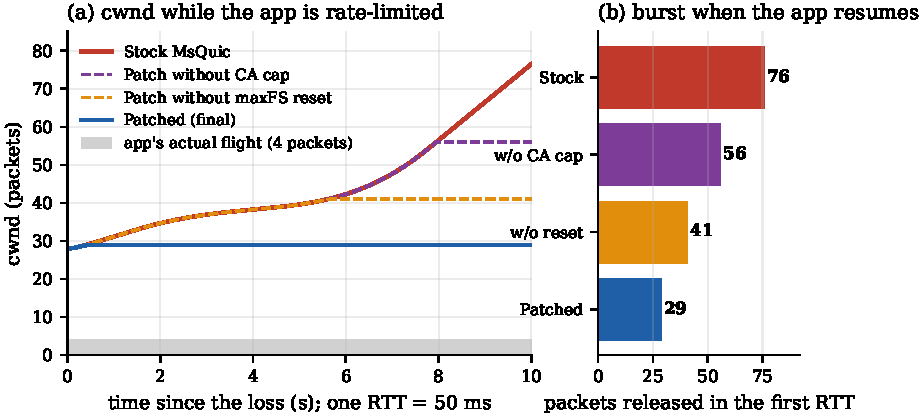
\includegraphics[width=\textwidth]{figures/scenario_a.pdf}
  \caption{Scenario A. (a) \cwnd\ during 200 rounds in which only 4 packets per
    round are sent. (b) Burst size in the first round after the application
    resumes. Both fixes are needed; each alone leaves a burst well above the
    40 packets at which the loss occurred.}
  \label{fig:scenA}
\end{figure}

\subsection{Scenario B --- why \ssthresh\ is not lowered (design decision)}
\label{sec:scenB}

\textbf{Setup.} Like A, but 20 of the 40 packets are lost, so the
re-measured $\maxfs = 20$ and the CA cap $20+1 = 21$ is \emph{below}
$\ssthresh = 28$. 40 rate-limited rounds, then 15 cwnd-limited rounds.

\textbf{What happens.} Figure~\ref{fig:scenB}. With the final patch, the cap
drops \cwnd\ to 21, the sender is then in slow start and the $2\cdot\maxfs$
cap lets \cwnd\ rise back to \ssthresh; the window moves between 21 and 28
and never exceeds \ssthresh. When the application resumes, the sender is
already in slow start and ramps to 31 packets in 15 rounds. With
\ssthresh\ lowered to 21, the window is flat during the rate-limited period
but the sender then grows by only one packet every two rounds, reaching 27.
The stock sender is at 34--36 throughout, above the 28 that \ssthresh\ says
is safe.

\begin{figure}[ht]
  \centering
  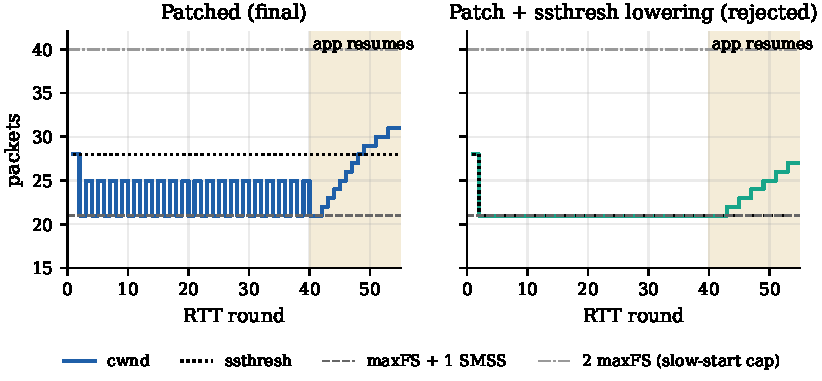
\includegraphics[width=\textwidth]{figures/scenario_b.pdf}
  \caption{Scenario B. Left: the final patch. Right: the rejected variant that
    lowers \ssthresh. The oscillation of the final patch stays below
    \ssthresh\ and costs nothing; lowering \ssthresh\ slows the later ramp-up.}
  \label{fig:scenB}
\end{figure}

\subsection{Scenario C --- a spurious loss is undone (C5)}

\textbf{Setup.} In congestion avoidance with $\cwnd \approx 29$ and a full
window in flight, 30\,\% of the flight is declared lost; then MsQuic learns the
loss was spurious and calls \texttt{OnSpuriousCongestionEvent}; then the rest
of the flight is acknowledged.

\textbf{What happens.} Figure~\ref{fig:scenC}. The undo restores \cwnd\ to
29.3 in every build. But C1 had set \maxfs\ to the post-loss flight of 21.
Without C5, the first ACK applies the CA cap $21+1 = 22$ and the undo is
silently cancelled: the sender loses 25\,\% of its window for a loss that
never happened. With C5, \maxfs\ is restored to 36 and the window continues
at 29.5, as in stock.

\begin{figure}[ht]
  \centering
  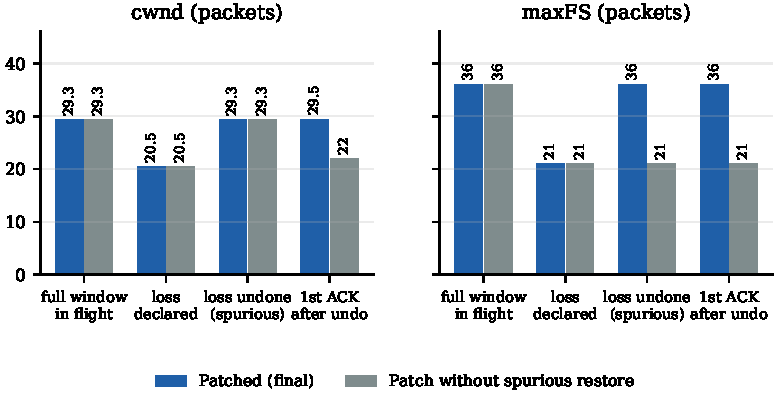
\includegraphics[width=0.85\textwidth]{figures/scenario_c.pdf}
  \caption{Scenario C. \cwnd\ and \maxfs\ at each step of a spurious loss and
    its undo. Without C5 the restored window is capped on the next ACK.}
  \label{fig:scenC}
\end{figure}

\subsection{Scenario D --- a heartbeat sender (C4 and the design decision)}
\label{sec:scenD}

\textbf{Setup.} After a loss at 40 packets, the application sends one 300-byte
heartbeat per round for 25 rounds; one heartbeat is lost. Then the application
starts a bulk transfer.

\textbf{What happens.} Figure~\ref{fig:scenD}(a): during the heartbeat phase
the stock window stays at 25\,861\,B (21 full packets) although the flight is
300\,B: when the bulk transfer starts it sends 20 packets at once. With the
draft rules the cap is $\maxfs + \smss = 300 + 1232$, which C4 raises to the
QUIC minimum window of $2\cdot 1232 = 2464$\,B. Without C4 the window falls
to 600\,B, \emph{smaller than one full-size packet}, which RFC~9002 forbids
and which costs the sender an extra round trip when it resumes.

Figure~\ref{fig:scenD}(b) shows the ramp-up when the bulk transfer starts.
The full patch slow-starts 2, 4, 8, 16 and reaches \ssthresh\ in four rounds,
then grows in congestion avoidance. The rejected \ssthresh-lowering variant
has \ssthresh\ at 2 packets and grows by one packet every two rounds: it
sends 9 packets in the 15th round instead of 23.

\begin{figure}[ht]
  \centering
  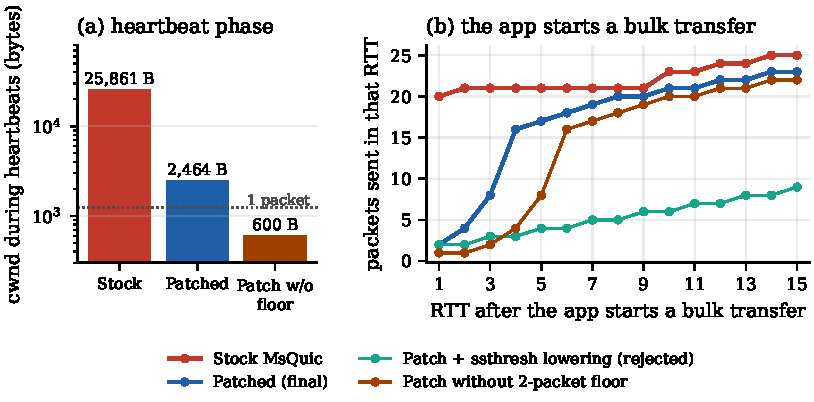
\includegraphics[width=\textwidth]{figures/scenario_d.pdf}
  \caption{Scenario D. (a) Window while one 300\,B heartbeat is sent per round
    (log scale). (b) Packets sent per round once the bulk transfer starts.}
  \label{fig:scenD}
\end{figure}

\subsection{Scenario E --- ECN (C1 and C2 on the ECN path)}

\textbf{Setup.} A 40-packet window is in flight; 20 packets have been
acknowledged when an ECN Congestion Experienced mark arrives. 100 rate-limited
rounds at 4 packets follow.

\textbf{What happens.} Table~\ref{tab:scenE}. ECN reduces the window from 60
to 42 packets in every build. The patched sender then re-measures \maxfs\ from
the 20 packets still in flight; the stock sender keeps 40. During the
rate-limited period the stock window keeps climbing the cubic curve to 56.6
packets. The patched window never exceeds \ssthresh\ (42) and ends at 37
(Figure~\ref{fig:scenE}). It moves between the CA cap and \ssthresh: each time
the cap drops \cwnd\ below \ssthresh, CUBIC is in slow start again, where the
draft allows up to $2\cdot\maxfs$. This is the bounded oscillation of
Section~\ref{sec:design}.

\begin{figure}[ht]
  \centering
  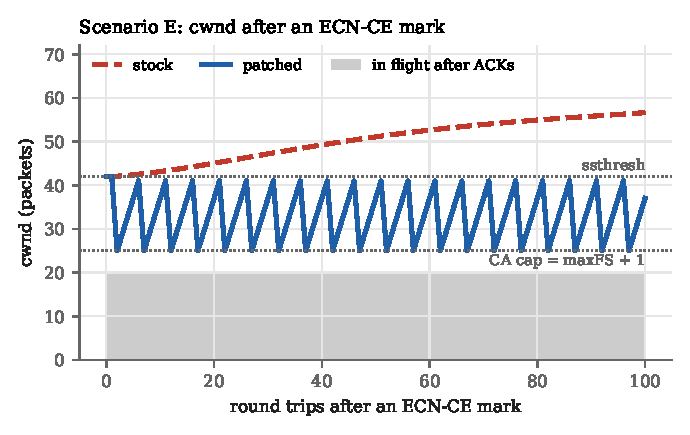
\includegraphics[width=0.62\textwidth]{figures/scenario_e.pdf}
  \caption{Scenario E. After the ECN mark, 20--24 packets stay in flight. Stock
    grows \cwnd\ along the cubic curve; the patch keeps it between
    $\maxfs + 1$ packet and \ssthresh.}
  \label{fig:scenE}
\end{figure}

\begin{table}[ht]
\centering
\caption{Scenario E (packets).}
\label{tab:scenE}
\begin{tabular}{@{}lcccc@{}}
\toprule
 & \cwnd\ before & \cwnd\ after & \maxfs\ after & \cwnd\ after 100 \\
 & ECN & ECN & ECN & rate-limited rounds \\
\midrule
\textcolor{stock}{stock}  & 60 & 42 & 40 & 56.6 (still growing) \\
\textcolor{patched}{full} & 60 & 42 & 20 & 37 (bounded by \ssthresh) \\
\bottomrule
\end{tabular}
\end{table}

%======================================================================
\section{An upstream bug found by the evaluation}
\label{sec:bug}

The first testbed campaign (Section~\ref{sec:sweep}) produced one result we
could not explain with the draft's rules: with a competing TCP flow, the
patched sender sometimes regrew its window after a loss at slow-start speed
while in congestion avoidance. The cause is a bug in MsQuic's CUBIC that is
independent of our patch and still present in upstream \texttt{main}.

\paragraph{Mechanism.} CUBIC keeps a Reno-friendly estimate
\texttt{AimdWindow} next to the cubic curve and uses
$\cwnd = \texttt{AimdWindow}$ whenever it is the larger one. The estimate
grows by one MSS each time an accumulator of ACKed bytes exceeds it:

\begin{lstlisting}[style=diff]
     if (Cubic->AimdAccumulator > Cubic->AimdWindow) {
-        Cubic->AimdWindow += DatagramPayloadLength;
-        Cubic->AimdAccumulator -= Cubic->AimdWindow;    // subtracts the GROWN window
+        Cubic->AimdAccumulator -= Cubic->AimdWindow;    // subtract the window crossed
+        Cubic->AimdWindow += DatagramPayloadLength;
     }
\end{lstlisting}

Both fields are \texttt{uint32\_t}. If the accumulator exceeds the window by
less than one MSS, which is the normal case for ACKs of one or two packets,
the subtraction wraps to about $4.3\times10^9$. From then on the condition is
true on every ACK, so \texttt{AimdWindow}, and with it \cwnd, grows by one MSS
per ACK: exponential growth in congestion avoidance. Congestion events reset
\texttt{AimdWindow} but not the accumulator, so the effect survives losses.
MsQuic's own test \texttt{AIMD\_AccumulatorTriggersWindowGrowth} chooses its
ACK size ``to avoid unsigned underflow in the subtraction'': the underflow
was known in the test, but not fixed in the code.

\paragraph{Evidence.}
\begin{itemize}
  \item \emph{Harness} (scenario F: loss, 10\,s rate-limited, resume, a second
        loss, then one ACK per packet). Stock MsQuic's accumulator wraps and
        \cwnd\ \emph{doubles every round} after the loss, from 89\,KB to
        2.8\,MB in five rounds (Figure~\ref{fig:bugF}). With the fix it grows
        by about 1\,KB per round, as CUBIC should.
  \item \emph{Real traces.} The signature of the bug is a congestion-avoidance
        increase of exactly one SMSS on one ACK. In stock MsQuic 11--33\,\% of
        all congestion-avoidance increases have it; with the fix, 0--6\,\%
        (Figure~\ref{fig:fourway}, lower left).
  \item \emph{Interaction with our patch.} Our cap $\maxfs + \smss$ does not
        stop this growth on a real network: every ACK lets the sender put one
        more packet in flight, which raises \maxfs\ and so the cap. Without the
        fix, our patch therefore still shows the signature in 2--24\,\% of
        increases.
\end{itemize}

\begin{figure}[ht]
  \centering
  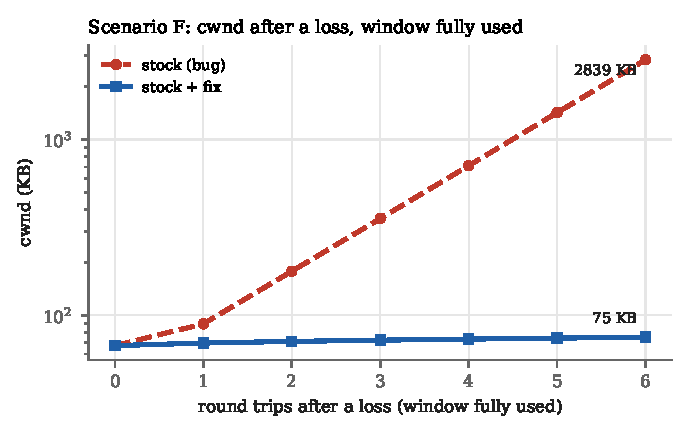
\includegraphics[width=0.62\textwidth]{figures/bug_harness.pdf}
  \caption{Scenario F, stock MsQuic with and without the accumulator fix. After a
    loss, with the window fully used and one ACK per packet, the wrapped
    accumulator makes \cwnd\ double every round trip in congestion avoidance.}
  \label{fig:bugF}
\end{figure}

\paragraph{Fix and test.} The two lines are swapped (msquic commit
\texttt{1ca13e9d7}, \texttt{patches/0004}). A new test,
\texttt{AIMD\_AccumulatorNoUnderflow}, crosses the window by 50 bytes and
fails on the old code; two tests that encoded the old order were updated.
Because the bug inflates stock MsQuic's numbers, we re-ran the key settings
with four builds to separate its effect from ours (Section~\ref{sec:fourway}).

%======================================================================
\section{Network evaluation}
\label{sec:net}

\subsection{Testbed and workload}

Linux network namespaces form a dumbbell (Figure~\ref{fig:topo}). The
bottleneck is the r1--r2 link, shaped by \texttt{netem} in both directions:
10\,Mbit/s by default, 20\,ms delay each way (base RTT 41\,ms), and a
100-packet drop-tail queue. Segmentation offloads (GSO, TSO, GRO) are turned
off on every interface, so the queue limit counts real packets: with UDP GSO
one queued buffer can hold many packets. A second client sends a ping every
10\,ms through the same bottleneck; in one setting it also runs a
long-lived TCP CUBIC flow (\texttt{iperf3}), started 3\,s before the QUIC
connection.

\begin{figure}[ht]
\centering
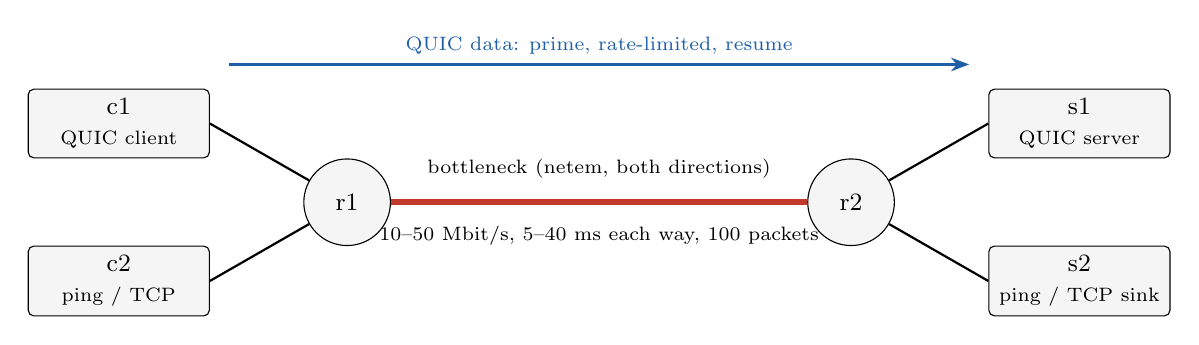
\begin{tikzpicture}[
  host/.style={draw, rounded corners=2pt, minimum width=2.3cm, minimum height=0.8cm,
               font=\small, align=center, fill=black!4},
  rtr/.style={draw, circle, minimum size=1.1cm, font=\small, fill=black!4},
  lk/.style={thick}]
  \node[host] (c1) at (0,1.0) {c1\\\scriptsize QUIC client};
  \node[host] (c2) at (0,-1.0) {c2\\\scriptsize ping / TCP};
  \node[rtr]  (r1) at (2.9,0) {r1};
  \node[rtr]  (r2) at (9.3,0) {r2};
  \node[host] (s1) at (12.2,1.0) {s1\\\scriptsize QUIC server};
  \node[host] (s2) at (12.2,-1.0) {s2\\\scriptsize ping / TCP sink};
  \draw[lk] (c1.east) -- (r1); \draw[lk] (c2.east) -- (r1);
  \draw[lk] (r2) -- (s1.west); \draw[lk] (r2) -- (s2.west);
  \draw[stock, line width=2pt] (r1) -- (r2);
  \node[font=\scriptsize, align=center, above=5pt] at (6.1,0) {bottleneck (netem, both directions)};
  \node[font=\scriptsize, align=center, below=5pt] at (6.1,0) {10--50 Mbit/s, 5--40 ms each way, 100 packets};
  \draw[-{Stealth}, patched, thick] (1.4,1.75) -- node[above, font=\scriptsize] {QUIC data: prime, rate-limited, resume} (10.8,1.75);
\end{tikzpicture}
\caption{Dumbbell topology. The QUIC client uploads to s1; c2's ping or TCP
  flow shares the bottleneck queue.}
\label{fig:topo}
\end{figure}

One QUIC connection runs three phases: \textbf{prime} (3\,MB as fast as
possible, so the window grows and meets losses as in normal operation),
\textbf{rate-limited} (6000\,B every 10\,ms, about 4.8\,Mbit/s, roughly
25\,KB in flight), and \textbf{resume} (8\,MB as fast as \cwnd\ allows).
Time~0 is the start of the 8\,MB transfer. We control how long the
application paces itself (250--3000 bursts, nominally 2.5--30\,s), but at 10\,Mbit/s the first
$\approx$5\,s of that are spent draining the 3\,MB prime. We therefore report
the time the sender was \emph{really} rate-limited, measured from its last
cwnd-limited send (flight $\ge 90\,\%$ of \cwnd) to resumption: 0, 0.7, 6, 17
and 28\,s for the five pacing lengths, the same in every build.

\paragraph{Campaigns and statistics.}
\begin{description}
  \item[Sweep] (Section~\ref{sec:sweep}): 11 settings (length of the
        rate-limited phase, RTT, bottleneck rate, competing TCP) $\times$ stock
        and patched $\times$ 10 runs = 220 runs.
  \item[Four builds] (Section~\ref{sec:fourway}): 5 settings $\times$ 4 builds
        $\times$ 10 runs = 200 runs. The builds are stock, stock + AIMD fix,
        ours, and ours + AIMD fix.
\end{description}
Runs are interleaved across settings and the build order rotates every
repetition, so slow drift of the machine cannot favour one build. We report
medians and quartiles, the difference of medians with a 95\,\% bootstrap
confidence interval, and a two-sided permutation test (20\,000 permutations).
All 420 runs completed.

\subsection{Sweep: stock vs.\ patched across settings}
\label{sec:sweep}

\begin{figure}[t]
  \centering
  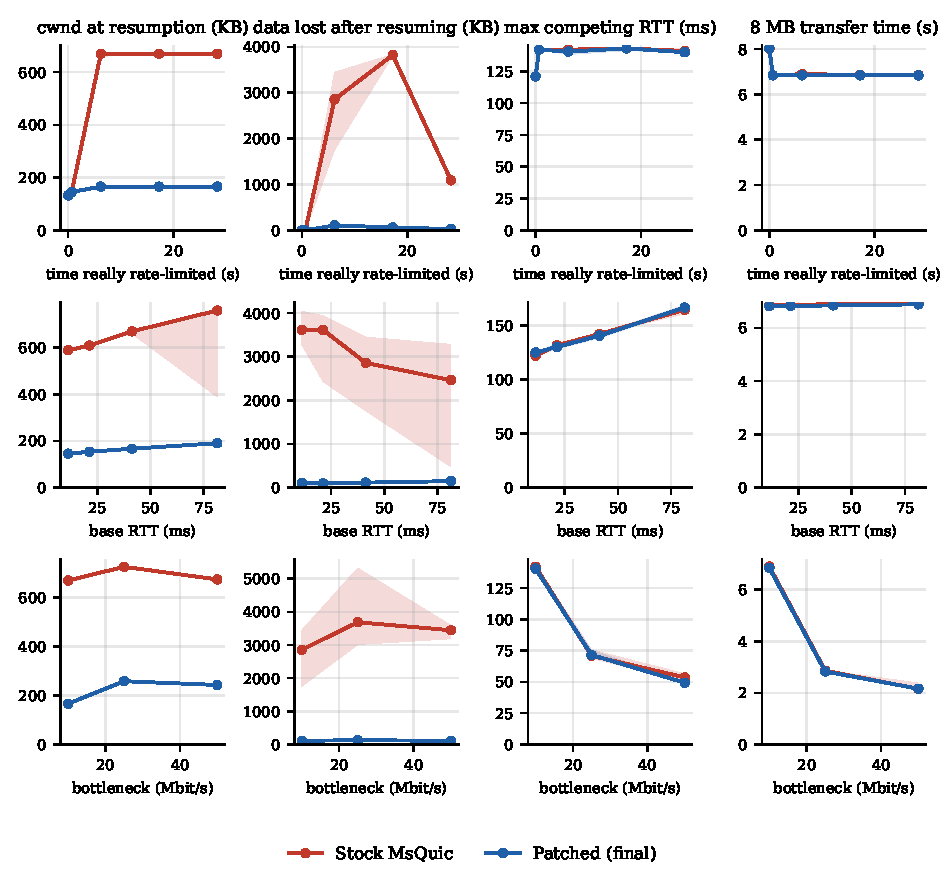
\includegraphics[width=\textwidth]{figures/sweep.pdf}
  \caption{Sweep campaign: medians (lines) and interquartile ranges (bands) over
    10 runs per point. Rows vary the length of the rate-limited phase, the RTT and
    the bottleneck rate; the other two stay at 6\,s, 41\,ms, 10\,Mbit/s. The
    $x$ axis of the first row is the measured time the sender was rate-limited.}
  \label{fig:sweep}
\end{figure}

\begin{table}[t]
\centering
\scriptsize
\caption{Sweep campaign, median stock / \textbf{patched}. $^{*}$: $p < 0.01$ (permutation test).}
\label{tab:sweep}
\setlength{\tabcolsep}{4pt}
\begin{tabular}{@{}llccccc@{}}
\toprule
Point & Bottleneck, RTT, & \cwnd\ at & lost after & max ping & 8\,MB & $n$ \\
 & rate-limited for & resume (KB) & resume (KB) & RTT (ms) & time (s) & \\
\midrule
\inputrows{tables/campaign_rows.tex}
\bottomrule
\end{tabular}
\end{table}

Figure~\ref{fig:sweep} and Table~\ref{tab:sweep} show three things.
\begin{itemize}
  \item \textbf{The harm needs time to build up.} With 0 and 0.7\,s of real
        rate-limited sending, CUBIC has not had time to grow the window and both
        builds behave the same. From 6\,s on, stock resumes with 590--760\,KB
        against 145--260\,KB for the patch, at every RTT and bottleneck rate.
  \item \textbf{The harm is loss, not delay.} Stock loses 1.1--3.8\,MB after
        resuming; the patch 31--145\,KB. With a real 100-packet queue the
        queueing delay is capped at about 120\,ms at 10\,Mbit/s, which both builds
        reach; the maximum ping RTT therefore differs by only a few
        milliseconds. (In an earlier, exploratory run with GSO enabled, where
        the effective queue was longer, the burst raised the competing RTT from
        43\,ms to a median maximum of 242\,ms with stock and 194\,ms with the
        patch, and up to 368 and 213\,ms in the worst runs; both builds there
        still had the accumulator bug.)
  \item \textbf{No cost in completion time} at 10--25\,Mbit/s: the 8\,MB
        transfer is as fast or slightly faster with the patch.
\end{itemize}
The competing-TCP setting was inconclusive, which led us to the bug in
Section~\ref{sec:bug}.

\subsection{Four builds: separating our change from the bug}
\label{sec:fourway}



\begin{figure}[t]
  \centering
  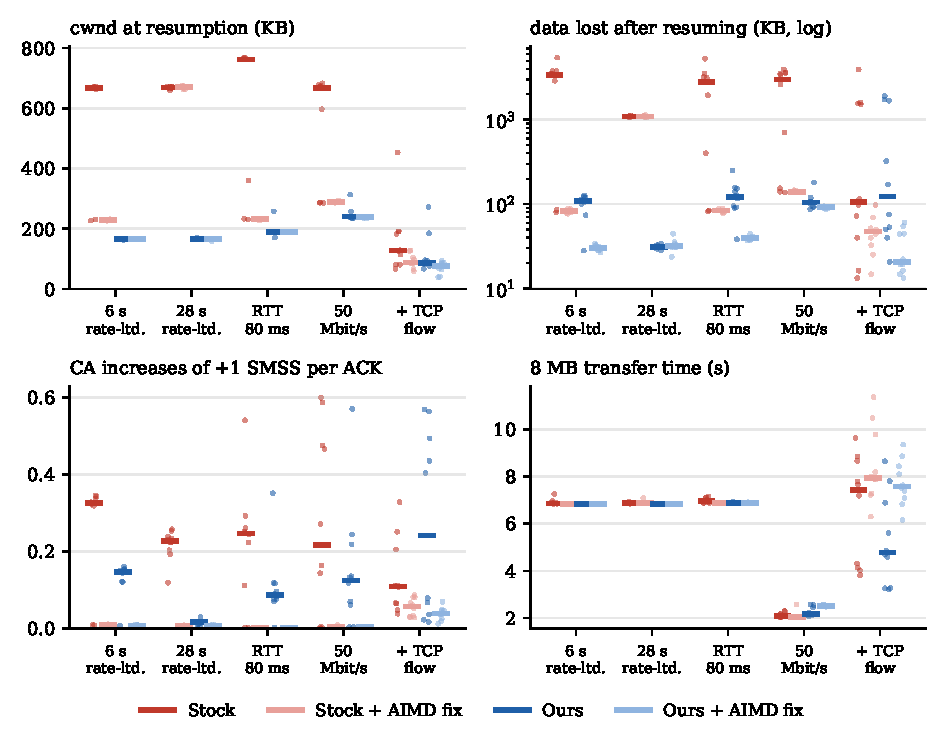
\includegraphics[width=\textwidth]{figures/fourway.pdf}
  \caption{Four builds, 10 runs each (dots) and medians (bars). Lower left:
    share of congestion-avoidance increases that are exactly one SMSS on one
    ACK, the signature of the accumulator bug.}
  \label{fig:fourway}
\end{figure}

\begin{table}[t]
\centering
\small
\caption{Four builds, medians over 10 runs. $p$: our change with the bug fixed in
  both builds (ours + fix vs.\ stock + fix).}
\label{tab:fourway}
\begin{tabular}{@{}llccccc@{}}
\toprule
Setting & Metric & Stock & Stock + fix & Ours & Ours + fix & $p$ \\
\midrule
\inputrows{tables/fourway_rows.tex}
\bottomrule
\end{tabular}
\end{table}

\begin{figure}[t]
  \centering
  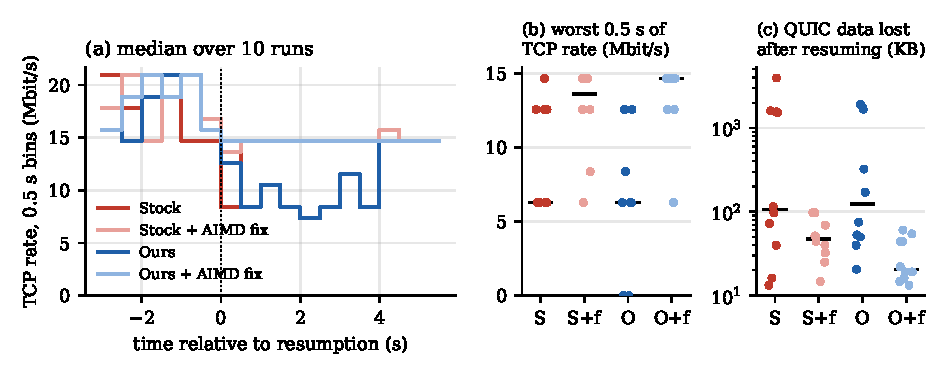
\includegraphics[width=\textwidth]{figures/fourway_compete.pdf}
  \caption{Competing TCP flow (25\,Mbit/s). (a) TCP rate around resumption,
    median of 10 runs; (b) worst 0.5\,s of TCP rate in the 2\,s after resumption;
    (c) QUIC data lost after resuming. S = stock, O = ours, +f = with AIMD fix.}
  \label{fig:compete}
\end{figure}

Table~\ref{tab:fourway}, Figures~\ref{fig:fourway}--\ref{fig:compete} and Figure~\ref{fig:hook} answer
the question the bug raised.
\begin{enumerate}
  \item \textbf{Most of stock's damage at 6\,s comes from the bug.} With the fix,
        stock resumes with 229 instead of 668\,KB and loses 82 instead of
        3413\,KB: the wrapped accumulator had pushed \cwnd\ up to the stale
        $2\cdot\maxfs$ limit in a few seconds.
  \item \textbf{After long rate-limited periods the draft's rule is what
        matters.} At 28\,s, the fix changes nothing (670\,KB, 1094\,KB lost):
        plain CUBIC reaches the stale limit on its own
        (Figure~\ref{fig:hook}). Our change cuts this to 166\,KB and 32\,KB,
        and the 8\,MB transfer is about 30\,ms faster.
  \item \textbf{With the bug fixed in both, our change still helps at every
        setting}: \cwnd\ at resumption $-17$ to $-28\,\%$ at 6\,s, RTT 80\,ms and
        50\,Mbit/s, and data lost after resuming $-34$ to $-63\,\%$
        (all $p < 0.001$).
  \item \textbf{Our change needs the fix.} With a competing TCP flow, ours
        without the fix is the worst build for TCP (median 11.0\,Mbit/s in the
        2\,s after resumption, worst 0.5\,s 6.3\,Mbit/s, three runs where TCP
        stalls completely for 0.5\,s), because the bug's per-ACK growth passes through
        the moving cap. Ours + fix is the best: 15.5 and 14.7\,Mbit/s, and the
        least QUIC data lost (21\,KB vs.\ 47\,KB for stock + fix, $p = 0.06$).
  \item \textbf{A cost on high-BDP paths with a shallow queue.} At 50\,Mbit/s
        the resumed burst overflows the 100-packet queue in all builds (first
        loss after 60\,ms). CUBIC then cuts to 70\,\% of the starting window and
        grows slowly from there, so starting lower (238 vs.\ 288\,KB) costs
        throughput: the 8\,MB transfer takes 2.5\,s instead of 2.0\,s and the
        first MB 52\,ms longer. This is the conservative side of the draft.
\end{enumerate}

%======================================================================
\section{Unit tests}
\label{sec:tests}

All 57 tests of MsQuic's \texttt{CubicTest} suite pass with the patches.
Table~\ref{tab:tests} lists the tests that were added or changed. Each new
test fails without the change it covers.

\begin{table}[ht]
\centering
\small
\caption{New and updated unit tests in \texttt{src/core/unittest/CubicTest.cpp}.}
\label{tab:tests}
\begin{tabularx}{\textwidth}{@{}>{\raggedright\arraybackslash\ttfamily\footnotesize}p{5.6cm} c X@{}}
\toprule
\normalfont\small Test & Change & What it checks \\
\midrule
RateLimited\_\-MaxFsResetOnLoss & C1, C2 &
  After losing 2400\,B out of 12\,320\,B in flight, \maxfs\ equals the remaining
  9920\,B, not the old peak. \\
RateLimited\_\-MaxFsResetOnEcn & C1, C2 &
  After an ECN mark, \maxfs\ equals the bytes still in flight. \\
RateLimited\_\-SpuriousCongestion\-RestoresMaxFs & C5 &
  A spurious-loss undo restores \maxfs\ to its pre-loss value. \\
RateLimited\_\-CongestionAvoidance\-CapIsMaxFsPlusSmss & C3 &
  After 30 ACKs in congestion avoidance with a constant flight,
  $\cwnd = \maxfs + 1232$. \\
SlowStart\_\-WindowOverflowAfter\-PersistentCongestion \normalfont(updated) & C3 &
  Previously asserted the old $2\cdot\maxfs$ limit; now asserts
  $\cwnd = \maxfs + \smss$. \\
HyStart\_\-ConservativeSlowStart\-Rounds\_TransitionToDone \normalfont(updated) & C3 &
  Asserts $\cwnd \le \ssthresh$ and $\cwnd \le 2\cdot\maxfs$ in slow start. \\
AIMD\_\-AccumulatorNoUnderflow & fix &
  The accumulator crosses \texttt{AimdWindow} by 50\,B; it must keep the 50\,B
  remainder and a further small ACK must not grow the window again. \\
AIMD\_\-AccumulatorTriggersWindowGrowth, AIMD\_\-SequentialLinearConvergence \normalfont(updated) & fix &
  Expected values follow the corrected order (subtract, then grow). \\
\bottomrule
\end{tabularx}
\end{table}

%======================================================================
\section{Discussion and limitations}
\label{sec:disc}

\begin{itemize}
  \item \textbf{Ship the bug fix with the patch.} The draft's cap
        $\maxfs + \smss$ bounds growth \emph{per measured flight}; on a real
        network the flight grows with every ACK, so a controller that grows by
        one packet per ACK (the accumulator bug) passes through it. Our patch
        without the fix was the worst build under competition
        (Section~\ref{sec:fourway}).
  \item \textbf{Conservative start on high-BDP paths.} When the resumed burst
        overflows a shallow queue anyway, a smaller starting window leads to a
        smaller window after the first loss, which CUBIC grows back slowly. At
        50\,Mbit/s with a 100-packet queue this cost 23\,\% in completion time of
        an 8\,MB transfer. Pacing the resumed burst would help both builds.
  \item \textbf{Loss, not delay.} With a real 100-packet queue the queueing
        delay is bounded by the queue, so the harm of the stock burst shows as
        loss (up to 3.8\,MB lost and up to ten times the bottleneck drops) rather than
        as extra latency for other flows. A longer queue (bufferbloat) would
        turn it into delay, as our exploratory GSO-enabled run showed.
  \item \textbf{Oscillation.} Without lowering \ssthresh, a rate-limited
        sender's window can move between $\maxfs + \smss$ and
        $\min(\ssthresh, 2\cdot\maxfs)$ (Scenario~B). This is bounded by
        validated values and was the better trade-off
        (Section~\ref{sec:design}).
  \item \textbf{Initial \maxfs.} The draft initialises \maxfs\ to the initial
        window; MsQuic initialises it to half of it, and we kept that. It only
        matters before the first window reduction, when it makes the
        slow-start cap $2\cdot\maxfs$ equal to the initial window until the
        flight exceeds half of it. Every result here is measured after a
        reduction, where the draft's reset applies.
  \item \textbf{Scope.} Only CUBIC is changed; MsQuic's BBR has its own
        application-limited handling. The cap uses the datagram payload size of
        path 0, like the rest of MsQuic's CUBIC, so it is not multipath-aware.
  \item \textbf{Testbed.} One emulated path with a drop-tail queue, one
        application pattern, at most one competing flow, 10 runs per point. The
        competing-TCP results are noisier than the others (bimodal outcomes),
        so differences there have wider intervals.
  \item \textbf{Scenario harness.} The scenarios use idealised whole-round ACKs.
        They isolate the logic of each change; the testbed covers network
        behaviour.
\end{itemize}

%======================================================================
\section{Conclusion}

A rate-limited sender should not be allowed to claim capacity it never used.
Stock MsQuic CUBIC already tried to enforce this, but its limit was based on
a stale maximum and was twice as loose as the draft allows in congestion
avoidance. With five small changes (34 lines of code) we implement the rules
of \texttt{draft-ietf-ccwg-ratelimited-increase-11}, and the ablation shows
where each change matters: C1--C3 stop the resumption burst (76 $\to$ 29
packets), C4 keeps the window legal for tiny flights, C5 keeps spurious-loss
undo working, and leaving \ssthresh\ alone keeps ramp-up fast.

The testbed evaluation also exposed an upstream bug, the underflow of CUBIC's
Reno-friendly accumulator, which inflated stock MsQuic's window and which our
change cannot contain on its own; we fixed it. With the fix in both builds,
our change removes the burst after long rate-limited periods (\cwnd\ 670
$\to$ 166\,KB, data lost 1094 $\to$ 32\,KB after 28\,s, $p < 0.001$), reduces
losses by 34--63\,\% after shorter ones and, together with the fix, keeps a
competing TCP flow's worst half-second at 14.7 instead of 6.3\,Mbit/s with
stock MsQuic. It costs no transfer time except on a high-BDP path with a
shallow queue.

%======================================================================
\begin{thebibliography}{9}
\bibitem{draft} M. Welzl, T. Henderson, G. Fairhurst, M. P. Tahiliani,
  \emph{Increase of the Congestion Window when the Sender Is Rate-Limited},
  IETF Internet-Draft \texttt{draft-ietf-ccwg-ratelimited-increase-11},
  September 2026.
\bibitem{rfc9002} J. Iyengar, I. Swett, \emph{QUIC Loss Detection and
  Congestion Control}, RFC~9002, 2021.
\bibitem{rfc9438} L. Xu, S. Ha, I. Rhee, V. Goel, L. Eggert, \emph{CUBIC for
  Fast and Long-Distance Networks}, RFC~9438, 2023.
\bibitem{rfc7661} G. Fairhurst, A. Sathiaseelan, R. Secchi, \emph{Updating TCP
  to Support Rate-Limited Traffic}, RFC~7661, 2015.
\bibitem{rfc5681} M. Allman, V. Paxson, E. Blanton, \emph{TCP Congestion
  Control}, RFC~5681, 2009.
\bibitem{msquic} Microsoft, \emph{MsQuic}, \url{https://github.com/microsoft/msquic}.
\end{thebibliography}

%======================================================================
\appendix

\section{Audit of the earlier plots in \texttt{experiments/}}
\label{app:audit}

Before this report, a number of exploratory plots had been made in
\texttt{experiments/}. We checked each against the raw data and the code.
None of them is used in this report. Every figure here was regenerated from
the raw traces by three scripts:
\begin{itemize}
  \item \path{report/make_figures.py},
  \item \path{experiments/analyze_campaign.py},
  \item \path{experiments/analyze_v3.py}.
\end{itemize}
The old plots are kept in \path{experiments/old_plots/}. Corrected versions of
the same ideas are drawn into \path{experiments/graphs/} by
\path{experiments/make_experiment_graphs.py}.

\begin{table}[H]
\caption{Verdict on each earlier plot in \texttt{experiments/}.}
\centering
\small
\begin{tabularx}{\textwidth}{@{}>{\raggedright\arraybackslash}p{4.6cm} l X@{}}
\toprule
Plot(s) & Verdict & Reason \\
\midrule
\texttt{gap1\_evidence\_clean(\_new)}, \texttt{gap1\_harm\_evidence} &
  correct & Show the stale \maxfs\ correctly, but not its consequence;
  superseded by \texttt{graphs/gap1\_before\_after.png}. \\
\texttt{resumption\_bomb*}, \texttt{bomb\_attempt} &
  invalid & Client and server logs interleaved in one series, producing
  vertical spikes; titles claim a burst the plotted data does not show. \\
\texttt{before\_cap\_comparison*}, \texttt{gap1/gap2\_after} &
  invalid & Caps computed from the plot title instead of the data, and from an
  earlier ``+1 byte'' version of the cap; \texttt{gap1\_after} is from a
  superseded build. \\
\texttt{appendix\_*}, \texttt{worked\_\-example}, \texttt{rls\_\-problem} &
  incomplete & Slow-start only (miss the CA rule) and mix bytes and packets
  on one axis; one has a 175\,s axis artefact. \\
\bottomrule
\end{tabularx}
\end{table}

\paragraph{Conventions in the new figures.} One colour per build throughout
(stock red, patched blue; lighter shades for the builds with the AIMD fix);
shared axes where panels are compared; units on every axis; the scenario
figures in packets of 1232\,B, the testbed figures in KB; every network figure
states the run it shows or how many runs it summarises; all figures are vector
PDFs.

\section{Reproducing the results}

\begin{lstlisting}[language=bash, style=c, morekeywords={}]
# apply the patches to upstream MsQuic 464c873c0
cd msquic && git am ../patches/*.patch
# unit tests
cmake --build build-test --target msquiccoretest
build-test/bin/Debug/msquiccoretest --gtest_filter='CubicTest.*'
# ablation (rebuilds cubic.c seven times, restores sources on exit)
report/ablation/run_ablation.sh
# harness: accumulator bug (scenario F), stock and stock + fix
report/ablation/run_f.sh stock > report/ablation/f_stock.txt
SRC=$PWD/report/ablation/cubic_stock_aimdfix.c \
  report/ablation/run_f.sh stockfix > report/ablation/f_stockfix.txt
# testbed campaigns (need root for network namespaces)
sudo experiments/run_campaign.sh        # sweep, 220 runs
sudo experiments/run_campaign.sh fix    # four builds, 200 runs
python3 experiments/analyze_campaign.py
python3 experiments/analyze_v3.py
python3 experiments/make_experiment_graphs.py   # experiments/graphs/
# figures and this document
python3 report/make_figures.py
python3 report/make_examples.py      # examples, bug_harness, scenario_e
cd report && tectonic report.tex
\end{lstlisting}

\end{document}
